%!TEX root = ../Physik I.tex

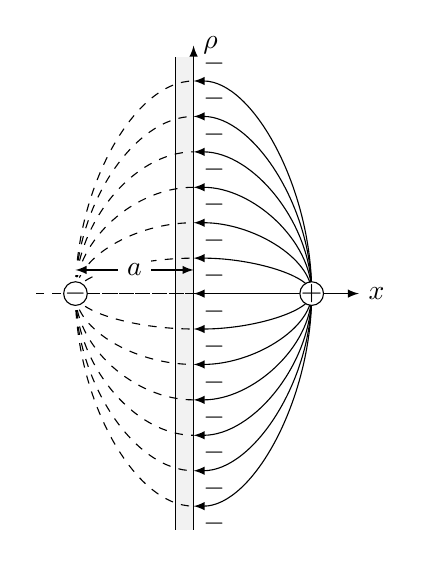
\begin{tikzpicture}[>=latex,scale=.3]
	% rest
	\begin{scope}
	\end{scope}
	
	% existing load
	\begin{scope}
		\draw[->] (0,0) -- (7,0) node[right] {$x$};
		
		\foreach \y in {.9,.75,...,-.9}
			\draw[yscale=\y,->] (5,0) .. controls (5,5) and (2.5,10) ..  (0,10);
		;
		
		\filldraw[fill=white]
			(5,0) circle (.5) node{$\footnotesize\boldsymbol{+}$}
		;
	\end{scope}
	
	% wall
	\begin{scope}
		\fill[fill=gray!10]
			(-.75,-10) rectangle (0,10)
		;
		\draw (-.75,-10) -- (-.75,10);
		\draw[->] (0,-10) -- (0,10.5) node[right]{$\rho$};
		
		\foreach \y in {9.75,8.25,...,-9.75}
			\draw (0,\y) node[right]{$\footnotesize -$};
		;
		
	\end{scope}
	
	% fictive load
	\begin{scope}
		\draw[dashed] (0,0) -- (-7,0);
		
		\foreach \y in {.9,.75,...,-.9}
			\draw[yscale=\y,dashed] (-5,0) .. controls (-5,5) and (-2.5,10) ..  (0,10);
		;
		
		\filldraw[fill=white]
			(-5,0) circle (.5) node{$\footnotesize\boldsymbol{-}$}
		;
		
		% distance a
		\begin{scope}[yshift=1cm]
			\fill[white] (-5.2,-.2) rectangle (-1,.2);
			\draw[<->] (0,0) -- (-5,0) node[pos=.5,fill=white]{$a$};
		\end{scope}
	\end{scope}
\end{tikzpicture}